% moduli_relationship.tex — K/G=2 -> nu=2/7 + the two longitudinal speeds (Vol 9 Ch.9)
% Pure TikZ schematic (no pgfplots): the elastic-identity chain and the KEEP-BOTH
% bulk-dilatation (sqrt2 c0) vs solid P-wave (sqrt(10/3) c0) speed distinction.
\begin{figure}[htbp]
\centering
\begin{tikzpicture}[
    box/.style={draw, rounded corners=3pt, align=center, font=\scriptsize, minimum height=0.85cm, inner sep=4pt},
    arr/.style={->, thick, gray},
    note/.style={font=\scriptsize, align=left}
]
    % top chain: K=2G (GR-imported operating point) -> nu_Hill = 2/7 (algebraic identity)
    % 🔴 K=2G PROVENANCE CORRECTION 2026-08-02 (CRIB-1; Rule 12 -- the prior node read "EMT at
    %   $p^* = 8\pi\alpha$\\$\Rightarrow K_{vac} = 2\,G_{vac}$" and the prior caption read "the EMT
    %   $K = 2G$ closure at $p^* = 8\pi\alpha$ fixes $\nu_{vac} = 2/7$"; both preserved verbatim
    %   here and in git). The figure DREW the superseded reading as a causal arrow: EMT => K=2G =>
    %   nu=2/7. Per ave-kb/vol3/gravity/ch01-gravity-yield/trace-reversal-mechanism.md:20-21 the
    %   EMT crossing is "a consistency illustration of the imported identity at the substrate
    %   operating point, not an independent determination of alpha or of K=2G", and per
    %   ave-kb/vol1/claim-quality.md:665 K=2G stays GR-imported at BOTH the Cauchy (PR #506) and
    %   micropolar (PR #508) grades. Fix shape: the K=2G box is re-labelled as the GR-imported
    %   operating point, the EMT crossing is drawn as what it is -- a DASHED consistency crossing
    %   INTO that box, not a derivation of it -- and only the K=2G -> nu_Hill arrow (which IS
    %   algebra) stays solid. nu_Hill anisotropy tag added per vacuum-poisson-ratio.md:18-24
    %   (PR #506). No speed, modulus or number changes; the KEEP-BOTH sqrt2-vs-sqrt(10/3) split
    %   below is untouched.
    \node[box, fill=blue!8] (kg) at (0,2.4) {$K_{vac} = 2\,G_{vac}$ operating point\\\scriptsize(GR trace-reversal; \textbf{value imported})};
    \node[box, fill=blue!8] (nu) at (5.4,2.4) {$\nu_{\mathrm{Hill}} = \dfrac{3K - 2G}{2(3K+G)}\Big|_{K=2G} = \dfrac{4}{14} = \dfrac{2}{7}$};
    \draw[arr] (kg.east) -- (nu.west);

    % EMT crossing: a CONSISTENCY illustration into the imported operating point, not a derivation
    \node[box, fill=gray!8, font=\scriptsize] (emt) at (0,3.9) {EMT crossing at $p^* = 8\pi\alpha$\\(consistency, not a determination)};
    \draw[arr, dashed] (emt.south) -- (kg.north);

    % two longitudinal speeds (KEEP-BOTH)
    \node[box, fill=green!10] (bulk) at (0,0.3) {\textbf{A1-dilatation port-mode}\\$v_{bulk} = \sqrt{K/\rho} = \sqrt{2}\,c_0$\\(drops the $4G/3$ shear term)};
    \node[box, fill=orange!12] (pwave) at (5.4,0.3) {\textbf{solid longitudinal P-wave}\\$c_L = \sqrt{(K + 4G/3)/\rho} = \sqrt{10/3}\,c_0$\\$\approx 1.83\,c_0$ (keeps the $4G/3$ term)};  % [DEMOTED 2026-08-11 --- R40-B2a: NEEDS RE-DERIVATION; dated note at the end of this file]

    \draw[arr] (kg.south) -- (bulk.north);
    \draw[arr] (nu.south) -- (pwave.north);

    % transverse speed
    \node[box, fill=gray!8] (vt) at (2.7,-1.6) {transverse / shear: $v_T = \sqrt{G/\rho} = c_0$ (photons by construction)};

    % distinction note
    \node[note, text width=4.4cm] at (10.0,1.3) {KEEP-BOTH (Rule 12, 2026-06-08 $c_L$ reconciliation): the two longitudinal speeds differ only by whether the $4G/3$ shear term is carried. Both are $\alpha$-free. $v_{bulk}$ is the bulk-modulus / A1-scalar quantity (\texttt{V\_LONG}); $c_L$ is the standard isotropic-solid P-wave at $\nu_{\mathrm{Hill}} = 2/7$ --- a $K = 2G$ re-expression that holds at the VRH average only, not a lattice-emergent ratio.};
\end{tikzpicture}
\caption{Moduli relationship chain (Vol.~9 Ch.~9 \S\ref{sec:vol9_mech_poisson}, \S\ref{sec:vol9_mech_wave_speeds}). The $K = 2G$ operating point is the GR trace-reversal identity --- form-derived, \textbf{value GR-imported} (\kbleaf{common/form-deriving-value-importing.md}); the EMT crossing at $p^* = 8\pi\alpha$ (dashed) is a \emph{consistency illustration} of that imported identity, not a determination of it (\kbleaf{vol3/gravity/ch01-gravity-yield/trace-reversal-mechanism.md}). Evaluating the isotropic elastic identity at $K = 2G$ then gives $\nu_{\mathrm{Hill}} = 2/7$ --- the isotropic Voigt--Reuss--Hill average, an averaging choice rather than a per-direction lattice output (Zener $A \approx 1.23$; \kbleaf{vacuum-poisson-ratio.md}). The two distinct longitudinal speeds — the A1-dilatation bulk-modulus port-mode $v_{bulk} = \sqrt{2}\,c_0$ vs the solid P-wave $c_L = \sqrt{10/3}\,c_0 \approx 1.83\,c_0$ — are kept separate (KEEP-BOTH, \texttt{clm-uu1qbo}). Canonical: \kbleaf{vacuum-poisson-ratio.md} (\texttt{clm-x19btt}); \kbleaf{constants.py} (\texttt{V\_LONG}).}
\label{fig:vol9_moduli_relationship}
\end{figure}
% --------------------------------------------------------------------------
% R40 batch-2a --- NEEDS-RE-DERIVATION status note (2026-08-11)
% --------------------------------------------------------------------------
% CLASS: status demotion under R40. Mints no clm-/def-/exp-/sup-/ilk-, moves no solidity number,
% adjudicates no channel and opens no fork. Every byte of each demoted claim is preserved; the
% stamped line gains a status marker only.
%
% THE ARC, IN FOUR CLAUSES (R40's header form; clause 4 points at the LANDED artifact, not at a
% ruling record). (1) The kill fired --- the walk-back that closed the bulk radiative-port
% reading. (2) The premise localized to the imported K = 2G elastic modulus: the compressible
% far-field branch was minted by a GR-imported modulus, not forced by the axioms. (3) The axioms
% underdetermine the bulk sector --- the flat-direction finding: the written action conserves the
% Gauss function pointwise and never fixes its value. (4) THE REPLACEMENT IS THE LANDED RATIFIED
% BOUND-SECTOR LAW --- AXIOM 5, SUBSTRATE DC BIAS, clauses S (deposit), G (bias coupling / bridge)
% and Q (quiescence), canonical at manuscript/common_equations/eq_axiom_5.tex with its register
% entry in manuscript/ave-kb/common/axiom-register.md. Under clause G the A1 / bulk slot is a
% BOUND RESPONSE --- u_0 = -A_g grad(eps_11), mechanism gloss BACK-REACTION --- with no
% independent propagating branch, no port and zero longitudinal characteristic speed. A bulk wave
% speed, a bulk radiative port, a bulk band-branch and a bulk transit clock therefore have no
% referent. A_g (the bias-coupling area) is an UNVALUED-RATIFIED-CONSTANT per R48
% (manuscript/ave-kb/common/interlock-register.md): it is not valued here or anywhere, and THE
% CALIBRATION COUNT STAYS 3.
%
% STANDING NAMED-OPEN DEBT (the honesty rider). The ratified axiom does NOT discharge everything.
% THE BIAS PROPAGATION THEOREM is Axiom 5's standing named-open debt, stated by the axiom's own
% phase-structure paragraph, clause (c1): clause G's elliptic law is the static abstraction of
% underived finite-speed bias dynamics, and the (u,pi) no-signalling theorem does NOT cover the
% bias read --- the bias's finite propagation speed is owed, not held. Every row tagged BIAS-DEBT
% below re-derives against the ratified axiom WITH THAT DEBT STANDING, never against a closed
% replacement.
%
% VOCABULARY. Canonical nouns authored here: the bound response (u_0), the bias (eps_11), the DC
% operating point / quiescent point (Q-point); back-reaction is the mechanism gloss. 'dress',
% 'grade' as eps_11's canonical noun, and 'halo' for the physics (the physics noun is the
% near-field store / added-mass) are RETIRED by R50; 'retardation' is retired by R49(b) in favour
% of propagation delay / finite propagation speed. Corpus text quoted below is byte-exact and is
% never reworded.
%
% ROWS CARRIED IN THIS FILE (verbatim quote + verbatim banked rationale):
%
%   :36  family: cross-volume ledger row (V_LONG / KEEP-BOTH)  [BIAS-DEBT]
%        QUOTE (byte-exact at HEAD): \textbf{solid longitudinal P-wave}\\$c_L = \sqrt{(K + 4G/3)/\rho} =
%        \sqrt{10/3}\,c_0$\\$\approx 1.83\,c_0$ (keeps the $4G/3$ term)
%       STAMPED AT: :36
%        RATIONALE (verbatim, research/drivers/r40_sweep_worklist_verified.json): Ledger-diagram of the
%        two phantom speed objects (:35 sqrt2*c_0 box, :36 P-wave box, KEEP-BOTH note :45): a figure
%        recording the imported reading's state; P-wave box void under the carve, sqrt2*c box re-scopes
%        to reflection-only — one re-keyed figure owed.
%        RESOLUTION: the demoted carrier is the propagating A1 / bulk branch; under Axiom 5 clause G that
%        slot is the bound response, so the re-derivation must be re-posed on the bound-sector
%        constitutive law (bias eps_11, bound response u_0, mechanism gloss back-reaction) rather than on
%        a compression wave. BIAS-DEBT: this row turns on finite-speed bias dynamics, so the resolution
%        is the ratified axiom WITH THE BIAS PROPAGATION THEOREM STANDING (clause (c1)) --- the
%        replacement is owed, not held.
%
% RECORDS: ruling R40 (the demotion sweep); the banked worklist
% research/drivers/r40_sweep_worklist_verified.json; the batch-0 scope verification and batch-1
% execution records in _orchestration/; this batch's record
% _orchestration/2026-08-12_r40-sweep-batch2a.md.
% --------------------------------------------------------------------------
